\begin{center}
  \Large\textbf{BIOGRAFI PENULIS}
\end{center}
\vspace{2ex}

\addcontentsline{toc}{chapter}{BIOGRAFI PENULIS}

\begin{wrapfigure}{L}{0.3\textwidth}
  \centering
  \vspace{-3ex}
  % Ubah nama file gambar berikut dengan nama file foto dari mahasiswa pertama
  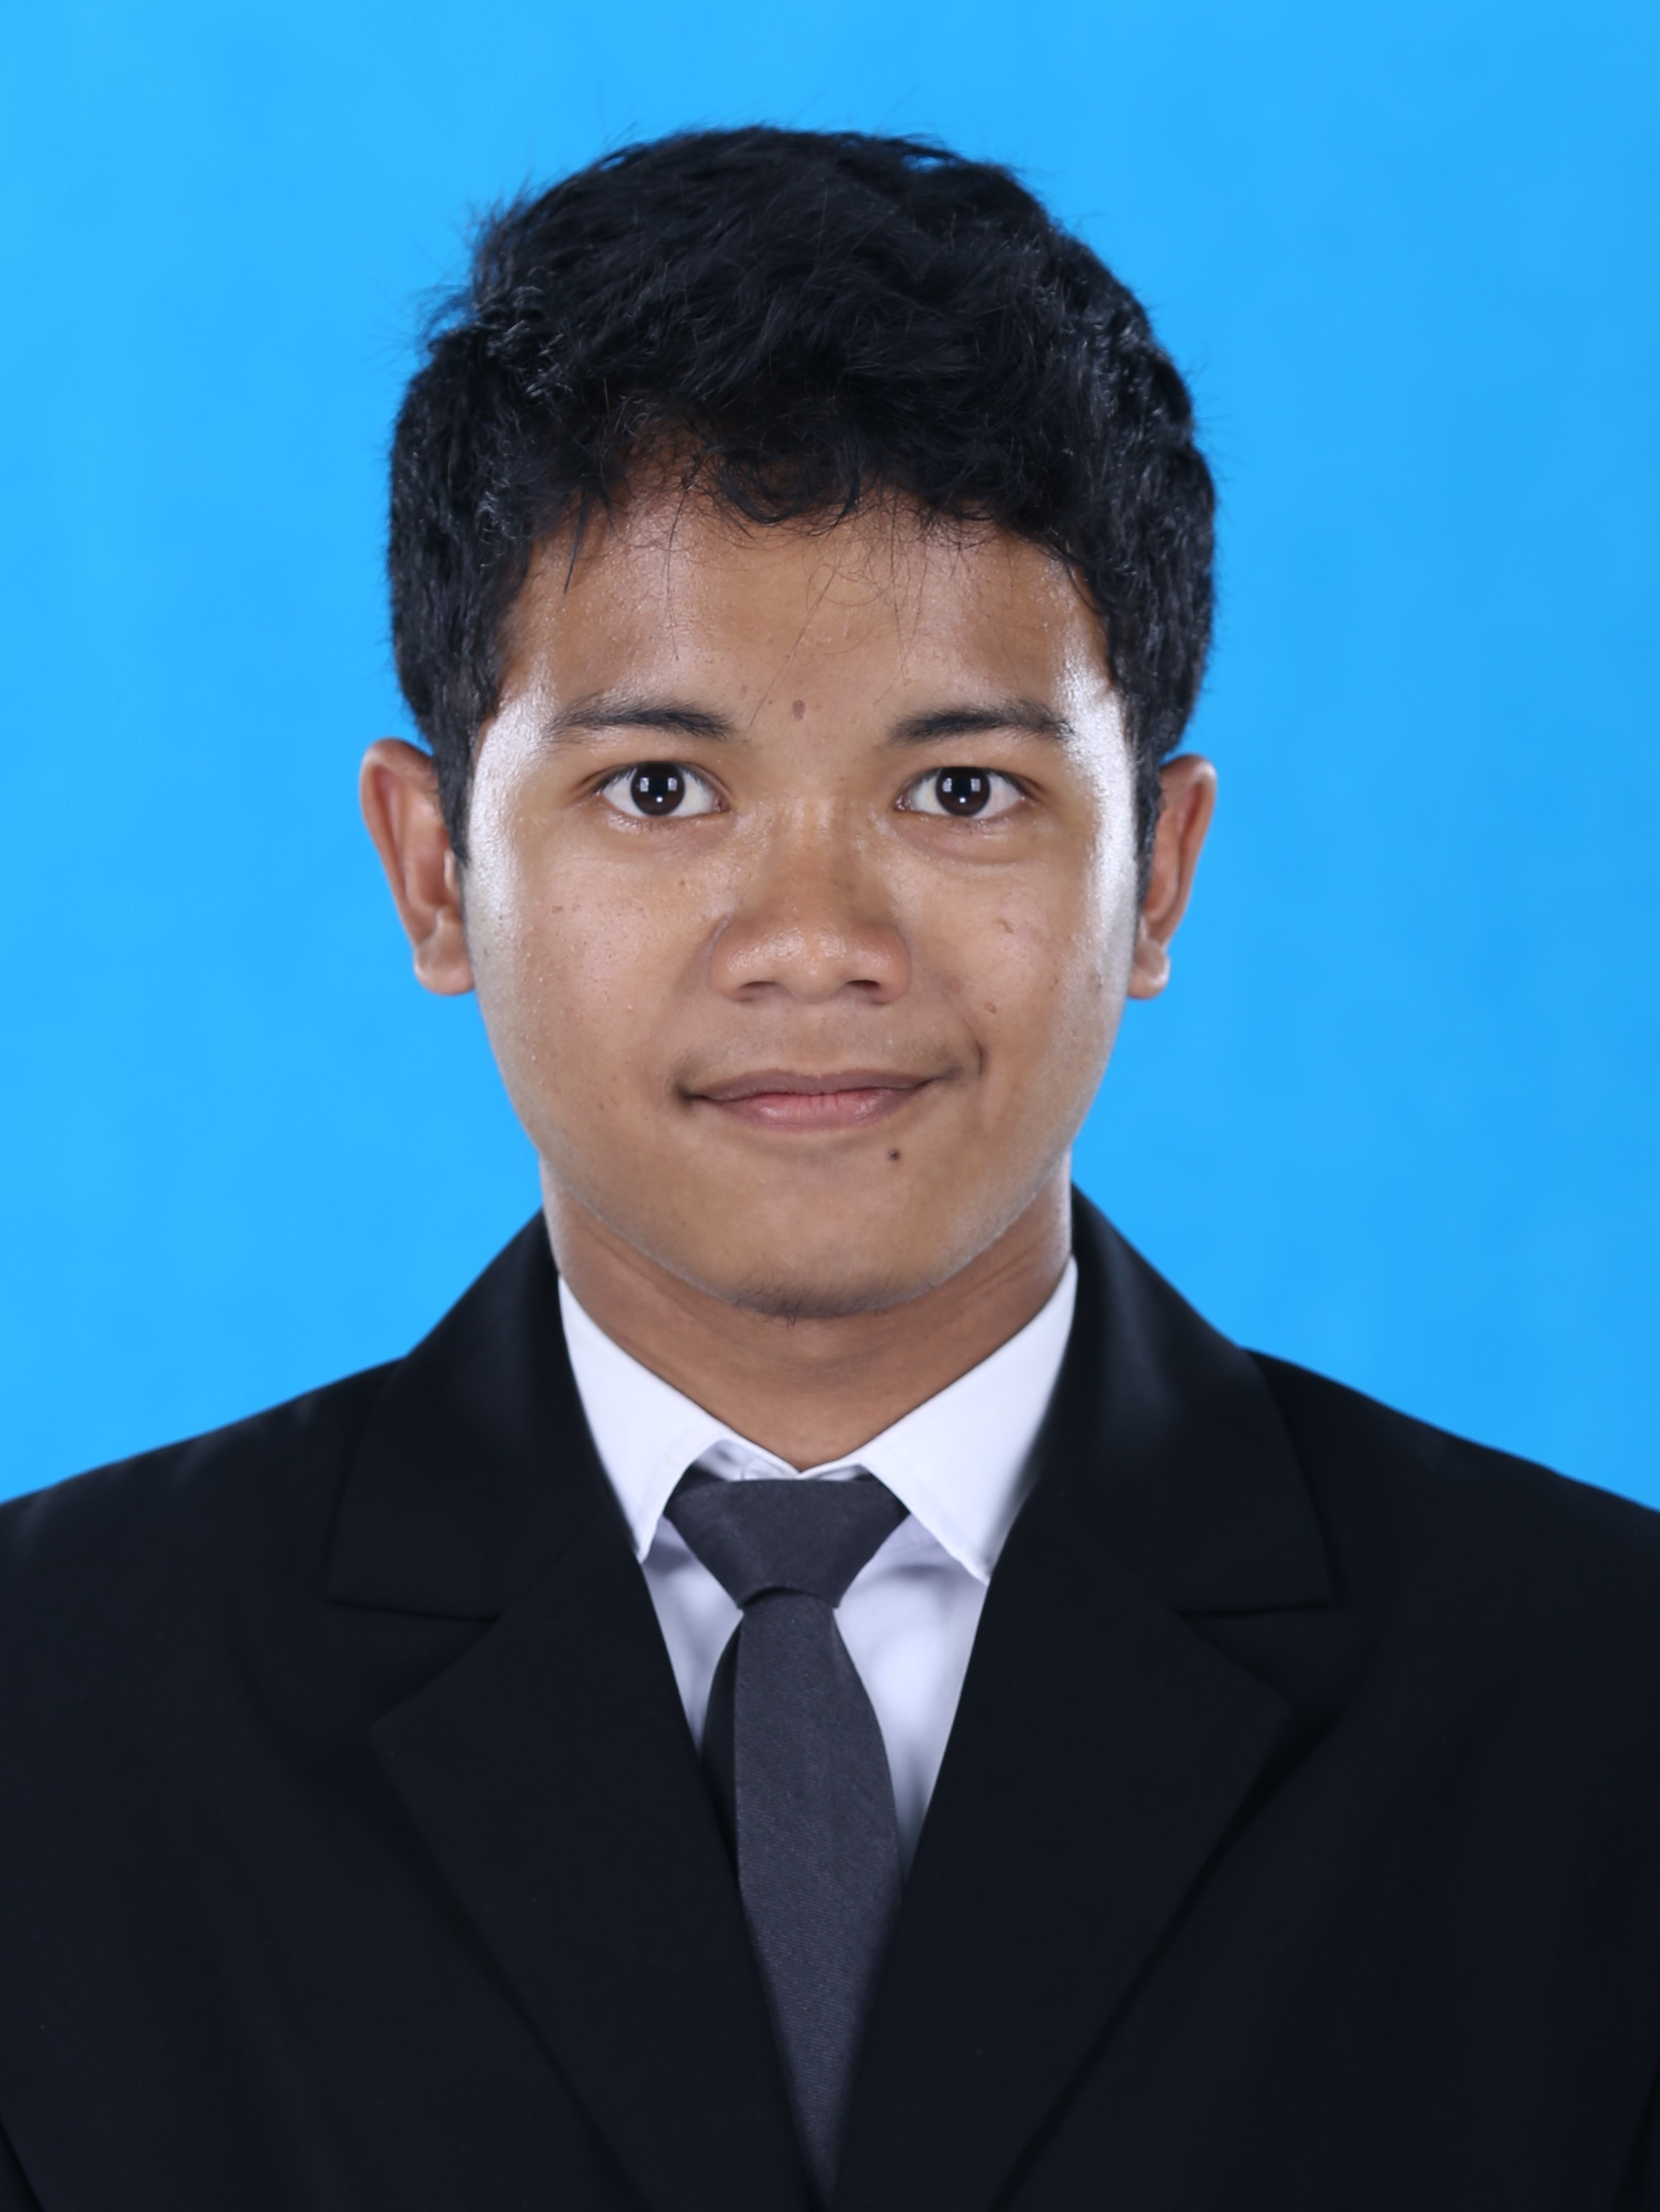
\includegraphics[width=0.3\textwidth]{gambar/ynw.jpg}
  \vspace{-4ex}
\end{wrapfigure}

% Ubah kalimat berikut dengan biografi dari mahasiswa pertama
\noindent Yusuf Nur Wahid, biasa dipanggil Ucup oleh teman-temannya lahir pada tanggal 18 Oktober 1998 di Banyuwangi.
Penulis memiliki riwayat pendidikan SDN 1 Cluring, SMPN 1 Cluring, SMAN 1 Genteng, dan S1 Teknik Komputer di ITS.
Selama kuliah penulis sempat menjadi asisten laboratorium \textbf{B201 Telematika} ITS pada periode 2019-2021.
Penulis juga memiliki hobi menulis kode karena menulis kode baginya adalah hal yang menyenangkan.
Apabila pembaca memiliki saran, kritik, ataupun pertanyaan mengenai laporan magang/kerja praktik ini dapat menghubungi penulis melalui \textit{email} \href{mailto:yusufedu@gmail.com}{yusufedu@gmail.com}.

\vspace{2ex}

\begin{wrapfigure}{L}{0.3\textwidth}
  \centering
  \vspace{-3ex}
  % Ubah nama file gambar berikut dengan nama file foto dari mahasiswa kedua
  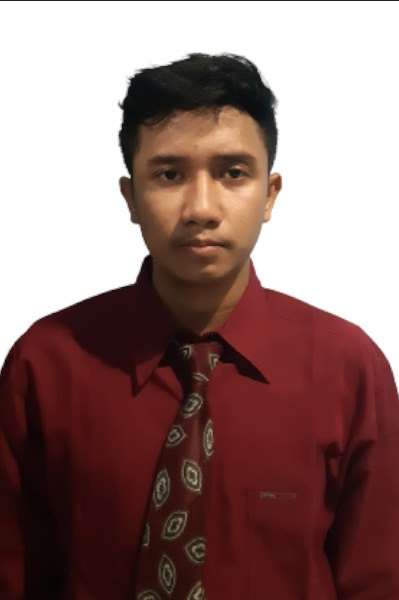
\includegraphics[width=0.3\textwidth]{gambar/helmika.png}
  \vspace{-4ex}
\end{wrapfigure}

% Ubah kalimat berikut dengan biografi dari mahasiswa kedua
\noindent Helmika Mahendra Priyanto, lahir tanggal 27 Desember 1999 di Mataram, Nusa Tenggara Barat.
Sedang menjalankan pendidikan di S1 Teknik Komputer ITS.
Penulis aktif dalam kegiatan lab dan organisasi mahasiswa di perguruan tinggi.
Penulis juga sering ikut dalam proyek pengembangan perangkat lunak dengan menggunakan bahasa \textbf{C}, \textbf{C++}, dan \textbf{C\#}.
Apabila pembaca memiliki saran, kritik, ataupun pertanyaan mengenai laporan magang/kerja praktik ini dapat menghubungi penulis melalui \textit{email} \href{mailto:helmika.zero@gmail.com}{helmika.zero@gmail.com}